\subsection{Problema de la mochila}

El problema de la mochila (\textit{knapsack}) consiste en seleccionar objetos con un valor \(v_i\) y un peso \(w_i\) para empacarlos en una mochila que tiene un límite de peso \(c\). La idea es maximizar el valor y solo se puede elegir cada objeto una vez.
\begin{especificacion}
  \entrada{arreglo de valores \(v\), arreglo de pesos enteros positivos \(w\) y capacidad de la mochila \(c > 0\).}
  \salida{valor máximo que es posible empacar.}
\end{especificacion}

\subsubsection{Subestructura óptima}

La subestructura óptima en este problema es relativamente evidente: el subproblema de empacar en la mochila solo un subconjunto de los objetos guarda exactamente la misma estructura que el problema general.
% Explicación más matemática

\subsubsection{Modelo}

Para formular una relación de recurrencia, la función \(f\) representa lo que se busca optimizar: el valor; en función de las variables de las que depende: los objetos que se consideran y la capacidad disponible.

Una forma de definir \(f(i, c)\) es como el valor óptimo posible para una capacidad de \(c\) cuando se seleccionan objetos entre los primeros \(i\). Esa es la \concept{formulación como prefijo}. La relación de recurrencia se obtiene relacionando el valor óptimo con la elección del iésimo objeto:
\begin{itemize}
  \item Si no se empaca el iésimo objeto, el valor \(f(i, c)\) es el mismo que se obtiene considerando solo los \(i-1\) objetos anteriores: \[f(i, c) = f(i-1, c)\].
  \item Si sí se empaca, el valor \(f(i, c)\) que se obtiene consiste en el valor \(v_i\) del objeto, más el máximo valor que se puede obtener de los \(i-1\) objetos anteriores usando no toda la capacidad disponible, sino \(c-w_i\) (pues hay que dejar espacio para el iésimo, que en este escenario sí se empaca): \[f(i, c) = v_i + f(i-1, c-w_i)\].
  \begin{itemize}
    \item Nótese que solo se puede elegir empacar el iésimo objeto si \(c \geq w_i\), de lo contrario no cabe.
  \end{itemize}
\end{itemize}
Con eso, la relación de recurrencia para la formulación como prefijo es
\[
f(i, c) = \begin{cases}
  f(i-1, c) & \text{si } c < w_i. \\
  \max\{f(i-1, c), v_i + f(i-1, c-w_i)\} & \text{si } c \geq w_i.
\end{cases}
\]
Los casos base son que no haya capacidad o un índice negativo: ninguno permite empacar objetos y por ende producen un valor de 0.

Análogamente, la \concept{formulación como sufijo} define \(f(i, c)\) como el valor óptimo con una capacidad \(c\) pero eligiendo entre los objetos desde el iésimo hasta el último. Ambas formulaciones son equivalentes, aunque hay a quienes alguna les parece más sencilla. La forma para obtener la relación de recurrencia es la misma:
\begin{itemize}
  \item Si no se empaca el objeto \(i\), el valor \(f(i, c)\) es el mismo que considerando desde el siguiente: \(f(i, c) = f(i+1, c)\).
  \item Si sí se empaca, se gana \(v_i\), pero al decidir si empacar desde el objeto \(i+1\) en adelante, solo se puede usar una capacidad de \(c-w_i\): \(f(i, c) = v_i + f(i+1, c-w_i)\).
\end{itemize}
A partir de eso:
\[
f(i, c) = \begin{cases}
  f(i+1, c) & \text{si } c < w_i. \\
  \max\{f(i+1, c), v_i + f(i+1, c-w_i)\} & \text{si } c \geq w_i.
\end{cases}
\]
Los casos base son, de nuevo, en los que no es viable empacar objetos y se obtiene un valor de 0: que no haya capacidad o que el índice exceda la cantidad de objetos.

Nótese que el caso base cambió por la definición de la función, ya no es un índice de 0, porque en la formulación como sufijo eso significa que quedan todos los objetos por empacar.

\subsubsection{Grafo de dependencias}

A diferencia de Fibonacci, aquí cada estado depende de dos variables, \(i\) y \(c\), por lo que el grafo de dependencias es bidimensional: cada fila corresponde a un valor de \(i\) y cada columna a un valor de \(c\). La figura \ref{fig:mochila_grafo_dependencias} lo ilustra para tres objetos con pesos \(w_0=2\), \(w_1=1\) y \(w_2=3\), y una capacidad máxima de \(4\).

Cada vértice \((i, c)\) tiene, cuando aplica, un arco horizontal desde \((i-1, c)\) (no empacar el objeto \(i\)) y un arco diagonal desde \((i-1, c-w_i)\) (sí empacarlo), de acuerdo con la relación de recurrencia. Los vértices de la fila \(i=-1\) son los casos base: no tienen predecesores.

\begin{center}
\setbox0=\hbox{%
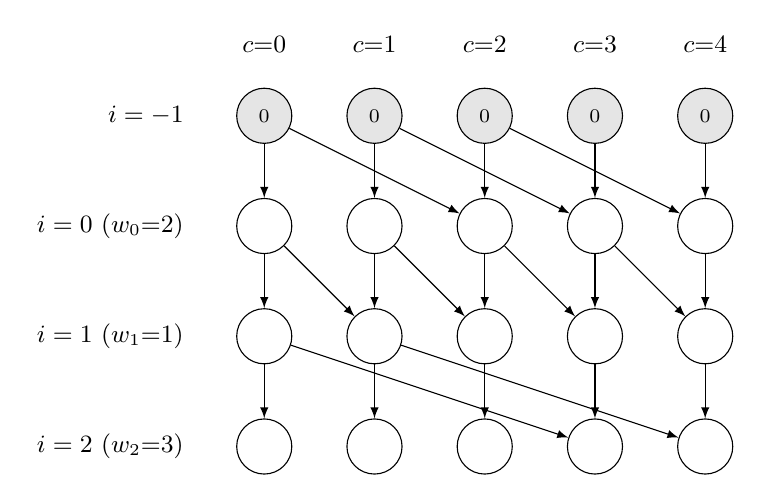
\begin{tikzpicture}[
  vertex/.style={circle, draw, minimum size=0.7cm, inner sep=0pt, font=\scriptsize},
  base/.style={vertex, fill=black!10},
  rowlbl/.style={font=\small, anchor=east},
  collbl/.style={font=\small},
  -latex,
]
  \foreach \c in {0,...,4} {
    \node[collbl] at (1.4*\c, 0.9) {\(c{=}\c\)};
  }

  \node[rowlbl] at (-0.9, 0)    {\(i=-1\)};
  \node[rowlbl] at (-0.9, -1.4) {\(i=0\) \((w_0{=}2)\)};
  \node[rowlbl] at (-0.9, -2.8) {\(i=1\) \((w_1{=}1)\)};
  \node[rowlbl] at (-0.9, -4.2) {\(i=2\) \((w_2{=}3)\)};

  \foreach \c in {0,...,4} {
    \node[base]   (nm1c\c) at (1.4*\c, 0)    {\(0\)};
    \node[vertex] (n0c\c)  at (1.4*\c, -1.4) {};
    \node[vertex] (n1c\c)  at (1.4*\c, -2.8) {};
    \node[vertex] (n2c\c)  at (1.4*\c, -4.2) {};
  }

  \foreach \c in {0,...,4} {
    \draw (nm1c\c) -- (n0c\c);
    \draw (n0c\c)  -- (n1c\c);
    \draw (n1c\c)  -- (n2c\c);
  }

  \draw (nm1c0) to (n0c2);
  \draw (nm1c1) to (n0c3);
  \draw (nm1c2) to (n0c4);

  \draw (n0c0) to (n1c1);
  \draw (n0c1) to (n1c2);
  \draw (n0c2) to (n1c3);
  \draw (n0c3) to (n1c4);

  \draw (n1c0) to (n2c3);
  \draw (n1c1) to (n2c4);
\end{tikzpicture}%
}
\ifdim\wd0>\textwidth
  \resizebox{\textwidth}{!}{\copy0}
\else
  \makebox[\linewidth]{\copy0}
\fi
\captionof{figure}{Grafo de dependencias de la mochila para tres objetos con pesos \(2\), \(1\) y \(3\), y capacidad \(4\). Los arcos horizontales representan no empacar el objeto de la fila y los diagonales, sí empacarlo.}
\label{fig:mochila_grafo_dependencias}
\end{center}

\subsubsection{Solución recursiva}

Cualquiera de las relaciones de recurrencia se pueden traducir inmediatamente a una implementación recursiva. La formulación como prefijo:
\begin{codeblock}[Mochila recursiva, formulación como prefijo.][impl:knapsack_recursivo]
\begin{pseudocode}
def recursive_prefix_knapsack(i: int, c: int) -> int:
    if i < 0: return 0

    value = recursive_prefix_knapsack(i-1, c)
    if c >= w[i]:
        value = max(value, recursive_prefix_knapsack(i-1, c - w[i]) + v[i])

    return value
\end{pseudocode}
\end{codeblock}

Y la formulación como sufijo:
\begin{pseudocode}
def recursive_suffix_knapsack(i: int, c: int) -> int:
    if i == n: return 0

    value = recursive_suffix_knapsack(i+1, c)
    if c >= w[i]:
        value = max(value, recursive_suffix_knapsack(i+1, c - w[i]) + v[i])

    return value
\end{pseudocode}

Naturalmente, ambas implementaciones tienen sentido dentro de una función principal que recibe todas las entradas del problema. Por ejemplo, para la formulación por prefijos.
\begin{pseudocode}
def recursive_knapsack(v: arreglo[int], w: arreglo[int], c: int) -> int:

    <implementación de recursive_prefix_knapsack>

    return recursive_prefix_knapsack(len(v)-1, c)
\end{pseudocode}

Nótese que, en ambas implementaciones, decidir sobre cada objeto es una decisión binaria: se empaca o no. Por ende, cada decisión duplica el árbol. La complejidad temporal es de \(O(2^n)\).

\subsubsection{Subproblemas superpuestos}

Nótese que distintas ramas de la recursión, o sea distintas decisiones sobre objetos anteriores, pueden conducir al mismo subproblema, es decir, a una llamada con los mismos valores de \(c\) e \(i\). Por lo tanto, existen problemas superpuestos. Eso hace que memoizar haga la solución más eficiente.

\subsubsection{Solución top-down}

Como el valor depende de dos variables, se debe usar una estructura bidimensional para memoizar los resultados, donde cada dimensión modela una variable. 

En este caso se usa una matriz (un arreglo de arreglos) donde la primera dimensión modela los objetos y la segunda modela la capacidad. Se reescribe la \hyperref[impl:knapsack_recursivo]{formulación recursiva como prefijo}, en gris, y se añaden en negro los pocos cambios necesarios para memoizar:
\begin{codeblock}[Mochila top-down (en gris: \hyperref[impl:knapsack_recursivo]{solución recursiva}).][impl:knapsack_top_down]
\begin{pseudocode}[style=derived]
def @top_down@_knapsack(v: arreglo[int], w: arreglo[int], c: int) -> int:
    @n = len(v)@
    @values = |\text{matriz de tamaño $n \times (c+1)$ llena de }|-1@

    def @top_down@_prefix_knapsack(i: int, c: int) -> int:
        if i < 0: return 0
        @if values[i][c] >= 0: return values[i][c]@

        value = @top_down@_prefix_knapsack(i-1, c)
        if c >= w[i]:
            value = max(value, @top_down@_prefix_knapsack(i-1, c - w[i]) + v[i])

        @values[i][c] = value@
        return value

    return @top_down@_prefix_knapsack(@n@-1, c)
\end{pseudocode}
\end{codeblock}

\subsubsection{Solución bottom-up}

La solución bottom-up consiste simplemente en diligenciar la matriz mediante ciclos, en lugar de a través de la recursión. Se emplea la formulación como prefijo que es más natural para llenarla en orden.

Como ya no habrá recursión, los casos base deben estar plasmados explícitamente en la matriz. Se crea de tamaño $(n+1) \times (c+1)$ para que la fila y la columna con índice \inline{0} representen los casos en los que no se puede empacar valor alguno: cuando solo se contemplan elementos anteriores al primero y cuando la capacidad es 0. Por ende, la primera fila no corresponde al primer objeto, sino a antes de empezar a empacar: pueden imaginarse los objetos como 1-indexados, como en la fórmula matemática, a pesar de no suele usarse en código; aunque al tabular, es muy útil y sí suele usarse.

% Seudodiagrama: la matriz, las filas son los objetos, las columnas son la capacidad desde 0 hasta c, la primera fila llena con 0 s.

\begin{pseudocode}
def bottom_up_knapsack(v: arreglo[int], w: arreglo[int], c: int) -> int:
    n = len(v)
    values = |\text{matriz de tamaño $(n+1) \times (c+1)$ llena de }|-1

    for i=0 to n:
        values[i][0] = 0
    for j=0 to c:
        values[0][j] = 0

    for i=1 to n:
        for j=1 to c:
            value = values[i-1][j]
            weight = w[i-1]  # -1 pq w es 0-indexed 
            if j >= weight:
                value = max(value, values[i-1][j-weight] + v[i-1])
            values[i][j] = value

    return values[n][c]  # O equivalentemente values[i][j]
\end{pseudocode}


\subsubsection{Optimización en espacio}


% \subsubsection{Solución bottom-up}

% Podemos incluso bajarle a la memoria

% Nótese que para calcular la fila \(i\) solo necesitamos la fila \(i-1\). Por ende, solo se necesitan guardar dos filas cada vez, las anteriores se pueden sobreescribir.

% Eso a su vez se puede achicar a una sola fila! Donde a la derecha está la fila de arriba y a la izquierda la de abajo.

% \subsubsection{}
    
% \end{annotations}
